\chapter{Elevation Map Generation}
\label{ch:elevation-map-generation}
When dealing with robot locomotion, the representation of the environment plays 
a fundamental role. It is, in fact, extremely important to properly
understand the structure of the world in order to safely make the robot move,
avoiding obstacles and dangerous zones, and to make it successfully complete 
its tasks. The world that surrounds the robot can be represented in many 
different ways; it is important to choose a proper representation to keep 
computational costs low and make to locomotion realizable.

In \textit{World of Stairs} scenarios, introduced in the previous chapter, the 
most efficient way to represent environments is by using elevation maps.
An elevation map is a grid that contains for each coordinate $(x, y)$ of the 
world its respective coordinate $z$. Hence, it can be seen as a function 
$\mathcal{M}_z$ such that, for each element $i$ of the grid,
$z_i = \mathcal{M}_z(x_i, y_i)$. This kind of representation allows the 
development of planners that quickly find plans to make robots move from a
position to another inside the world. 

This chapter introduces \texttt{elevation\_mapping}
\cite{Fankhauser2018ProbabilisticTerrainMapping}, the framework used in this 
thesis to generate elevation maps, which allow NAO to navigate in unknown 
environments (more precisely in \textit{World of Stairs} environments);
the ASUS Xtion Pro, an RGB-D sensor equipped on top of NAO, which has been 
used to send depth informaton to \texttt{elevation\_mapping}; 
the behaviour of the framework when a map is build using the ASUS Xtion Pro
placed on the head 
of NAO humanoid robot. The generated map is the one used in the experiment 
``Stair Climbing in Unknown Environment'', described in Section
\ref{sec:stair-climbing-unkenv}, and it is used by the footstep planner (Chapter
\ref{ch:rrt-based-footstep-planning}) to make NAO climb the stairs.

\section{Framework}
\texttt{elevation\_mapping} \cite{Fankhauser2018ProbabilisticTerrainMapping}
is a framework that allows to create elevation maps 
in rough environments using proprioceptive localization and distance sensors 
of the robot in real-time. The generated map is robot-centric,
meanining that the map is a local representation of the environment that 
surrounds the robot. Using a robot-centric representation instead of a 
world-centric one (where the map is expressed with respect to an inertial 
frame) has the advantage of not depending on the global pose of the robot.
This allows to avoid problems related to drift in the state estimation 
which would cause the maps 
to be inconsistent and not accurate enough to be used for locomotion.

The framework represents the map as a grid, providing for each cell a 
probabilistic distribution of the height of the terrain in the 
corresponding position. The map is updated using range measurements, provided 
by a sensor mounted on the robot, and the motion of the robot,
provided by a localization module such as a Kalman filter.
The program supports dynamic environments and it is built in C++, providing 
a ROS \cite{ros-melodic} interface which makes it simple to be integrated with
external sensors and other programs. \texttt{elevation\_mapping} is built 
upon GridMap \cite{Fankhauser2016GridMapLibrary}, which efficiently manages 
2D grid representations.

Even if not all the characteristics of the framework have been used in this 
thesis, the choice to integrate \texttt{elevation\_mapping} into the project 
has been essential to quickly build elevation maps that can be used by a
footstep planner (Chapter \ref{ch:rrt-based-footstep-planning}). Moreover, its 
versatility (because of the ROS interface) and its capabilities to generate 
efficiently maps for rough and dynamic environments, set a good starting point 
to extend this project to more complex scenarios. This section gives a brief 
overview of the framework without describing all the features in detail,
thoroughly described in \cite{Fankhauser2018ProbabilisticTerrainMapping}.

\subsection{Definitions}
The notation of the reference frames used by the framework are illustrated in 
Fig. \ref{fig:elevationmapping-coords-illustration}. In particular, $I$ is the 
inertial frame, $B$ is the base frame, $S$ is the sensor frame and $M$ is the 
map frame. The inertial frame $I$ is considered to be fixed with respect to the 
terrain. Both the base frame $B$ and the sensor frame $S$ are attached to the 
robot and it is assumed that the transformation $(r_{BS}, \Phi_{BS})$ between 
the two is known in advance. The elevation map is attacched to  
the reference frame $M$. $B$ and $M$ are related through a transformation 
$(r_{BM}, \Phi_{BM})$ given by the user. The $z$ axis of the map frame $M$ and 
the inertial frame $I$ are always aligned. A cell $i$ of the elevation map 
corresponding to the point of the surface $P_i = (x_i, y_i, \hat{h}_i)$,
which is expressed 
with respect to $M$. The transform $(r_{IB}, \Phi_{IB})$ between the position
of the robot $B$ and the 
inertial frame $I$ is provided by a state estimation module.
\begin{figure}
  \centering
  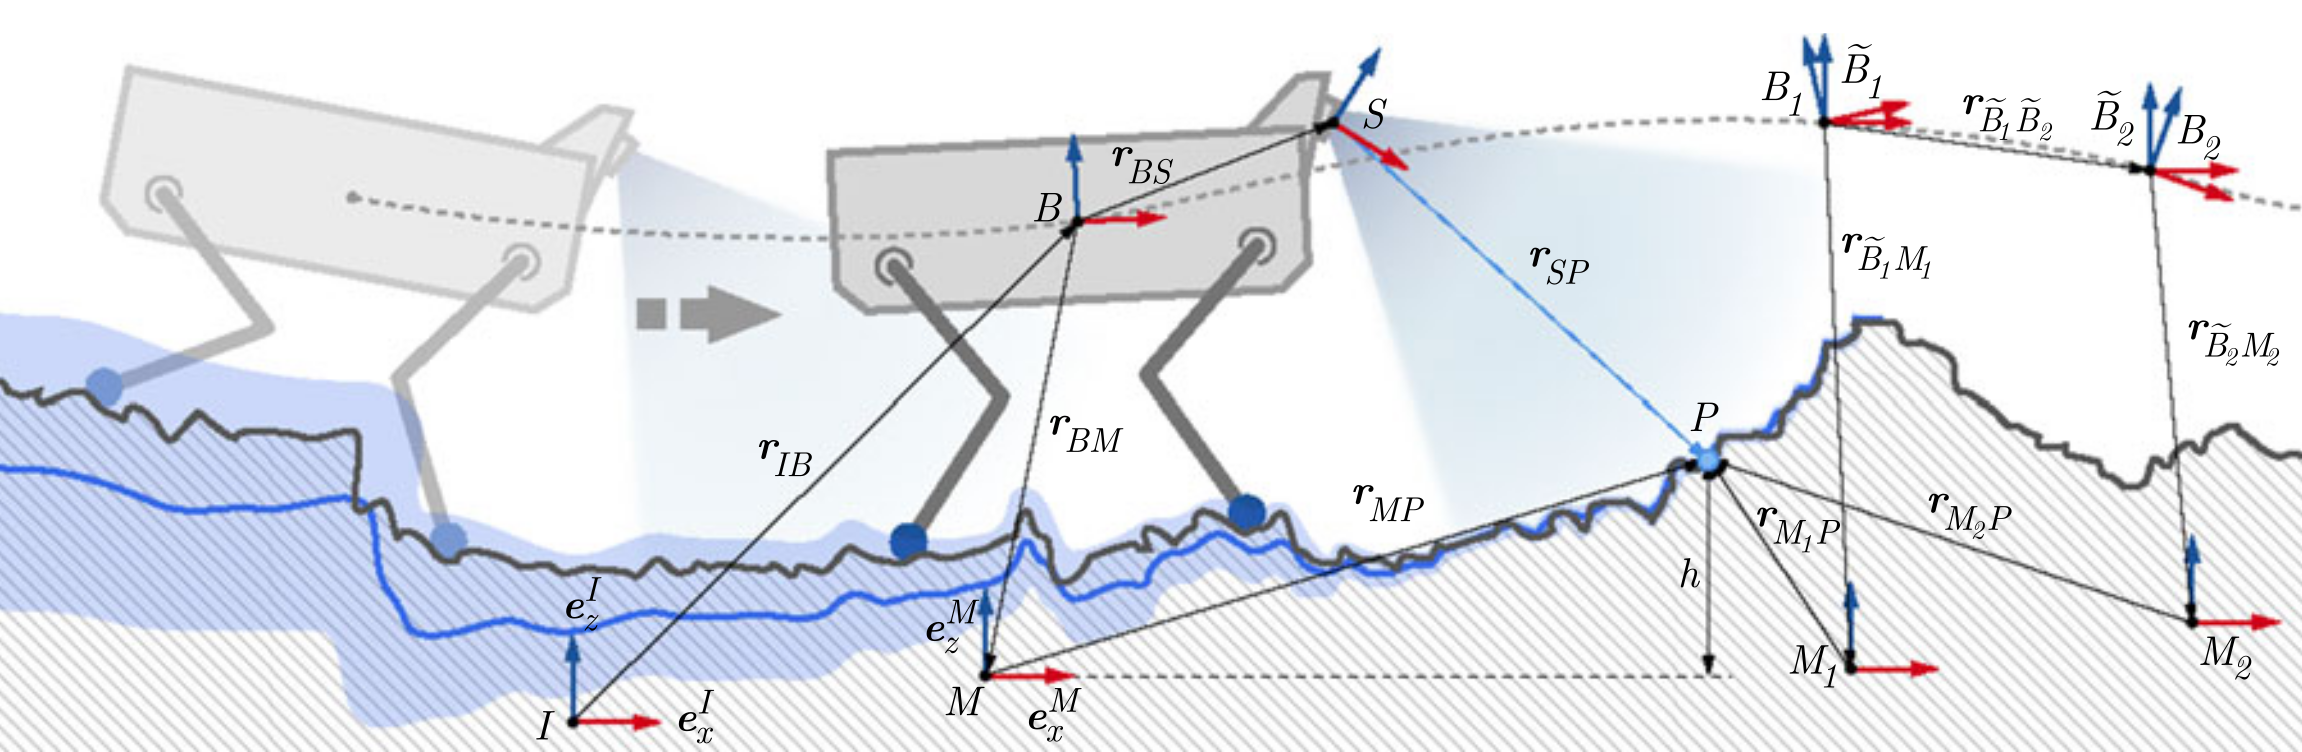
\includegraphics[width=\textwidth]
      {figures/elevationmapping-coords-illustration.png}
  \caption{The figure shows the notation of the reference frames used by 
      \texttt{elevation\_mapping}.
      \cite{Fankhauser2018ProbabilisticTerrainMapping} together with the 
      robot moving inside a rough environment.}
  \label{fig:elevationmapping-coords-illustration}
\end{figure}

\subsection{Map Update}
The map is updated when new measurements are read by the distance sensor and 
when the localization module updates the position of the robot. Each 
measurement $\tensor[_S]{r}{_{SP}}$ in the sensor frame $S$ is first transformed 
into the corresponding height measurement $p$ using the kinematic 
representation described before (Fig.
\ref{fig:elevationmapping-coords-illustration}).
The new height measurement can be represented as a Gaussian probability
distribution $\tilde{p} \sim \mathcal{N}(p, \sigma_p^2)$ given the sensor noise 
model \cite{Fankhauser2015Kinectv2}. In this way, it is possible to update 
the current estimate of the height $\mathcal{N}(\hat{h}, \sigma_h^2)$ by using 
a 1D Kalman filter, obtaining a new estimate of the height
$\mathcal{N}(\hat{h}^{+}, \sigma_h^{2+})$. The filter is updated only if the 
new measurement is not too far away (in terms of Mahalanobis distance)
from the current estimate.

The height estimate of each cell needs to be updated also during motion in 
order to take  
into account the uncertainty of the motion itself. To speed up the process,
each cell $i$ is extended with a spatial covariance matrix $\Sigma_{P_i}$ that,
in addition to the uncertainty of the height $\sigma_{h_i}^2$,
considers the uncertainty along the $x$ and $y$ axes.

\subsection{Map Fusion and Dynamic Environments}
The map fusion step is performed whenever required and it consists in 
transforming the elevation map data from a probabilistic representation of the 
kind $\mathcal{N}(\hat{h}_i, \Sigma_{P_i})$ to a deterministic representation 
$(\hat{h}_i, h_{i,\min}, h_{i,\max})$, where the values $h_{i,\min}, h_{i,\max}$
respectively represent the lower and the upper bound of the height estimation 
such that $h_i$ has 95\% probability of being in the range $[h_{i,\min},
h_{i,\max}]$. In this thesis the fused map is used by the footstep planner 
(Chapter \ref{ch:rrt-based-footstep-planning}) to generate a plan for the robot,
similarly to \cite{Fankauser2018RobustRoughTerrainLocomotion}.

\texttt{elevation\_mapping} handles dynamic environments by performing a 
visibility check based on ray tracing. Since this is a computationally 
expensive task, it is performed in parallel to the data acquisition process and 
it is run at a low frequency~(1 Hz).

\section{ASUS Xtion Pro}
The camera (Fig. \ref{fig:asus-xtion-pro}) used in this thesis is an
ASUS Xtion Pro \cite{ASUSXtionProWebsite},
which is equipped with a depth sensor, used to generate the height measurements
sent to \texttt{elevation\_mapping}. The communication between the camera and 
the mapping framework is handled by ROS.
ASUS Xtion Pro works up to a resolution of $640\times480$
at 30 fps. Its working range is from 0.5m up to 3.5m. The camera has been 
calibrated with a tool called \texttt{camera\_calibration}
\cite{cameracalibrationros}.
\begin{figure}
  \centering
  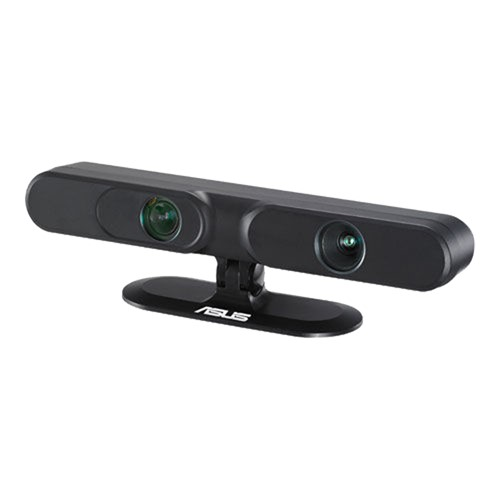
\includegraphics[width=0.5\textwidth]{figures/asus-xtion-pro.jpeg}
  \caption{The ASUS Xtion Pro \cite{ASUSXtionProWebsite} is equipped with a
      depth sensor and it is 
      easily configurable to make it work with ROS. This simplifies the 
      integration with \texttt{elevation\_mapping} and, consequently, 
      the construction of a navigable map.}
  \label{fig:asus-xtion-pro}
\end{figure}

\section{World of Stairs}
The integration between \texttt{elevation\_mapping} and the ASUS Xtion Pro 
allows to easily generate elevation maps in rough environments, meaning that 
the same settings could be used to generate elevation maps for \textit{World 
of Stairs} scenarios, described in the previous chapter.

As mentioned before, ROS simplifies the communication between the camera and 
the mapping framework, allowing to develop a block scheme (Fig.
\ref{fig:block-scheme}) that connects the camera to the robot. The humanoid 
robot used in this thesis is NAO, shown in Fig. \ref{fig:nao-with-xtion}
where it has been equipped with the ASUS Xtion Pro.

The \textit{World of Stairs} scenario considered for the experiments is the one 
shown in Fig. \ref{fig:nao-with-xtion-full-env}, where the robot stands in 
front of a stairway. The idea is to position the camera towards the stairs in 
order to generate an elevation map accurate enough to be used by a footstep
planner (Chapter \ref{ch:rrt-based-footstep-planning}). Given the pose of the 
camera, which is sent to \texttt{elevation\_mapping} together with the depth 
information of the camera, it is possible to quickly generate a map.
Of course, the area underneath the robot can not be seen by the camera. That is 
why a ``safe zone'' is manually added to the final elevation map before 
sending it to the planner.
Fig. \ref{fig:onlymap-xtion-20cm} shows the map generated by the framework 
(together with the ``safe zone'') when the 
camera is oriented towards the stairs (as in Fig. \ref{fig:xtion-rgb-20cm}).
The generated map is the one used by the footstep planner in the scenario 
``Stair Climbing in Unknown Environment'', described in Section
\ref{sec:stair-climbing-unkenv}, where NAO is able to climb the stairs in an 
unknown environment.
\begin{figure}
  \begin{subfigure}[b]{0.49\textwidth}
    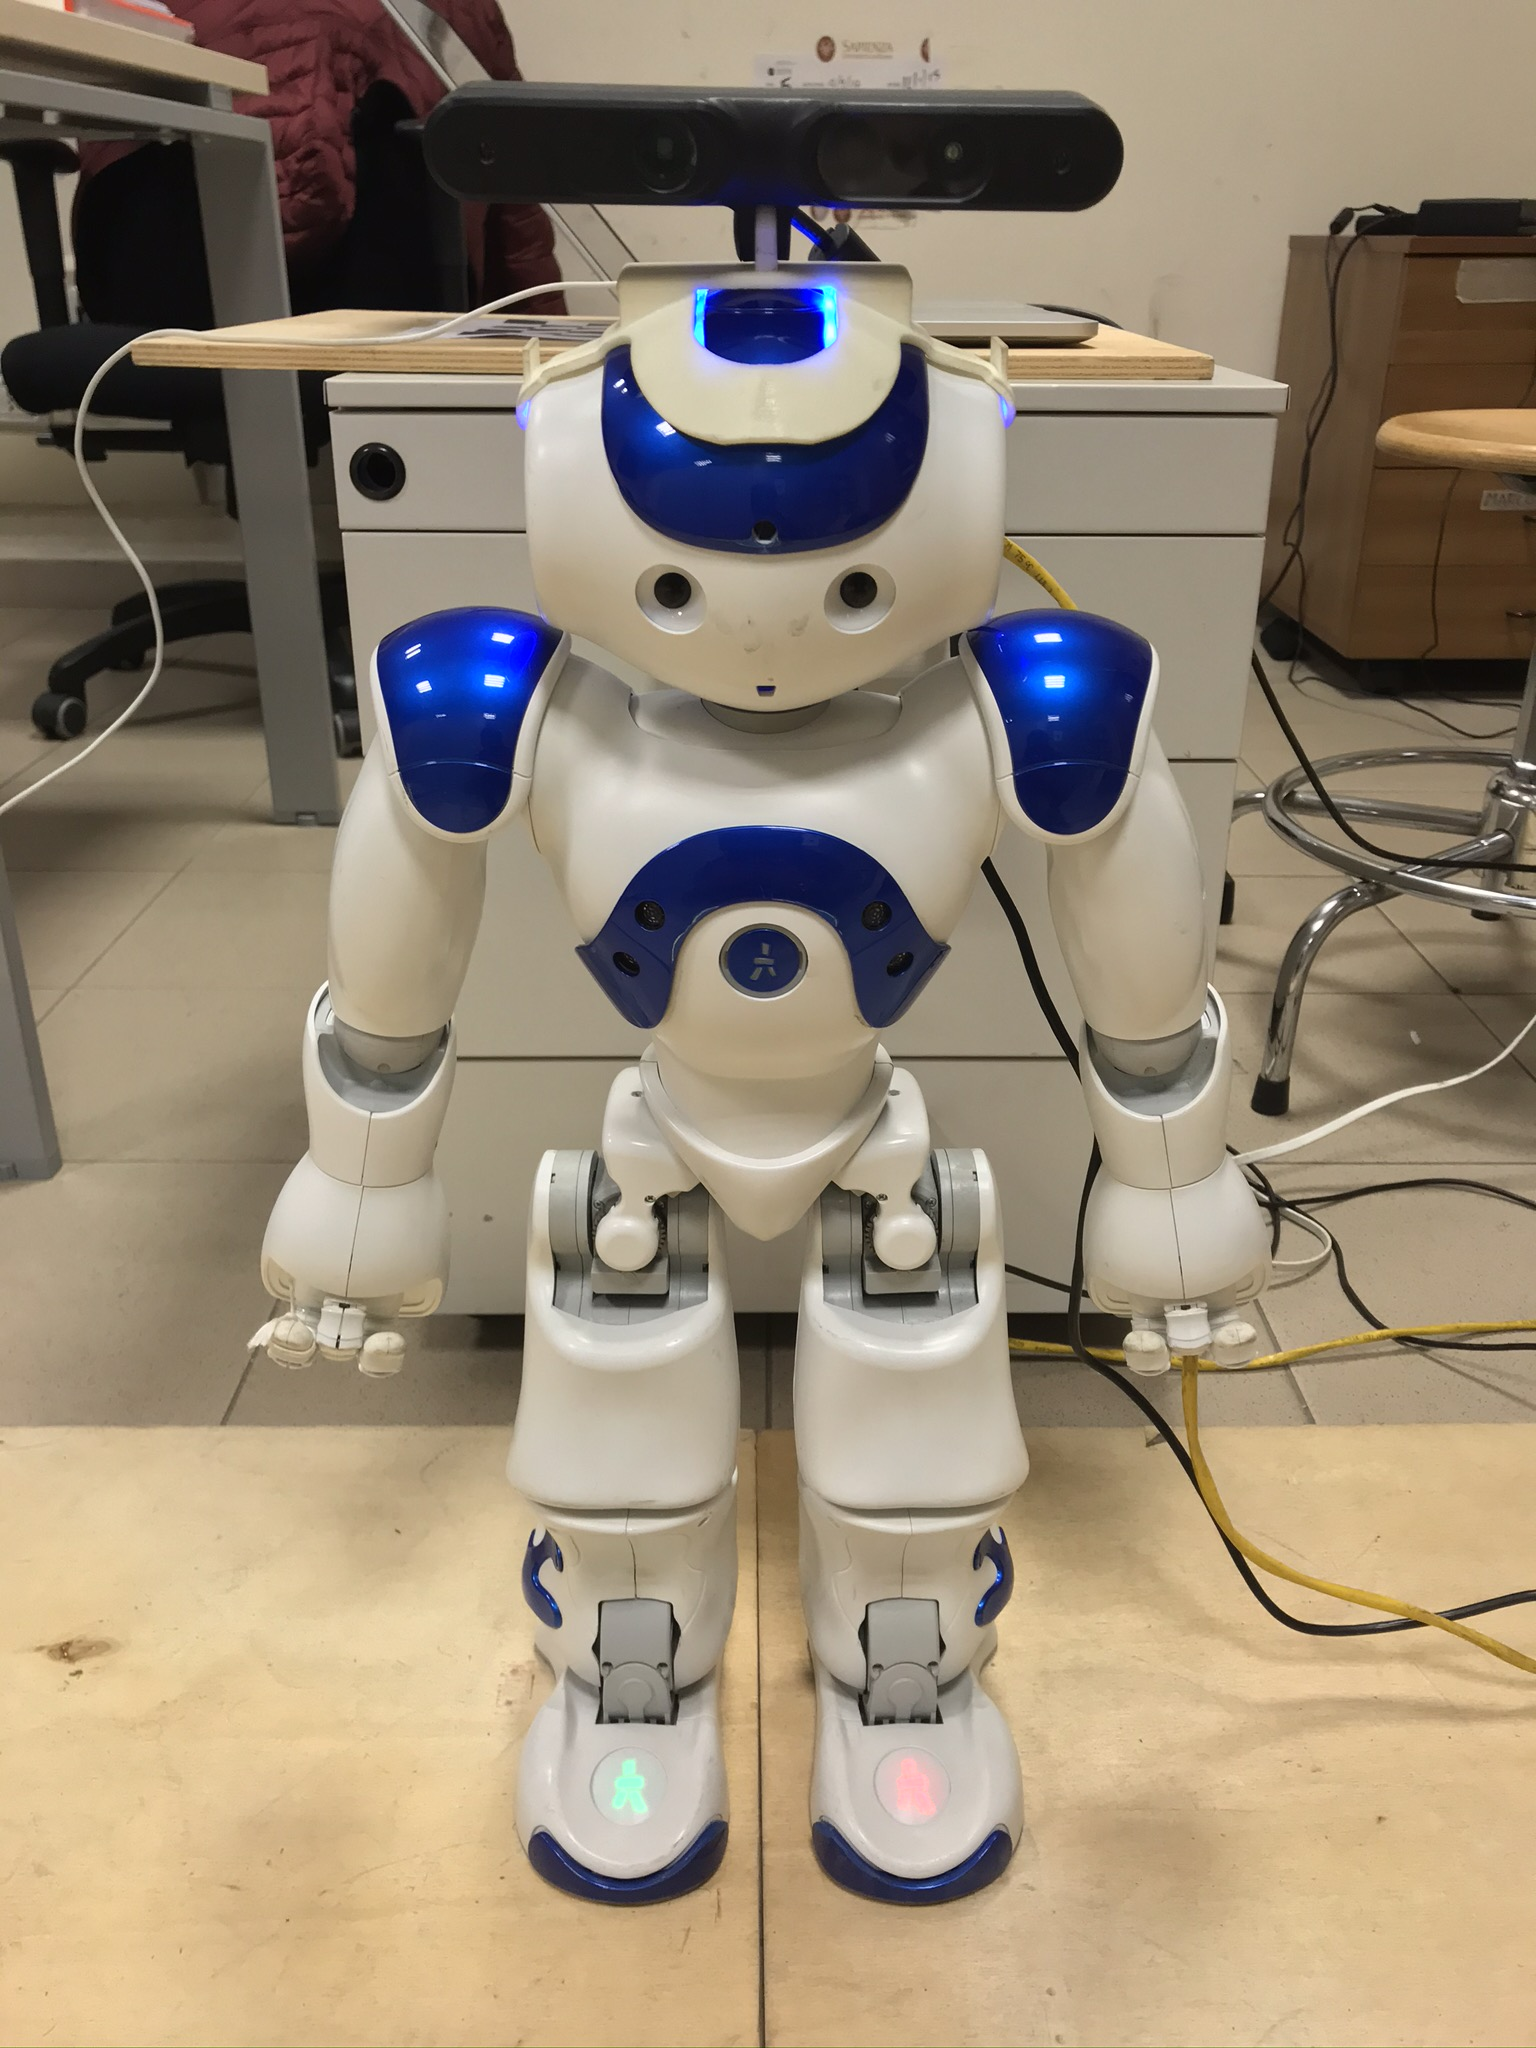
\includegraphics[width=\textwidth]{figures/NAO-with-xtion.JPEG}
    \caption{}
    \label{fig:nao-with-xtion}
  \end{subfigure}
  \hfill
  \begin{subfigure}[b]{0.49\textwidth}
    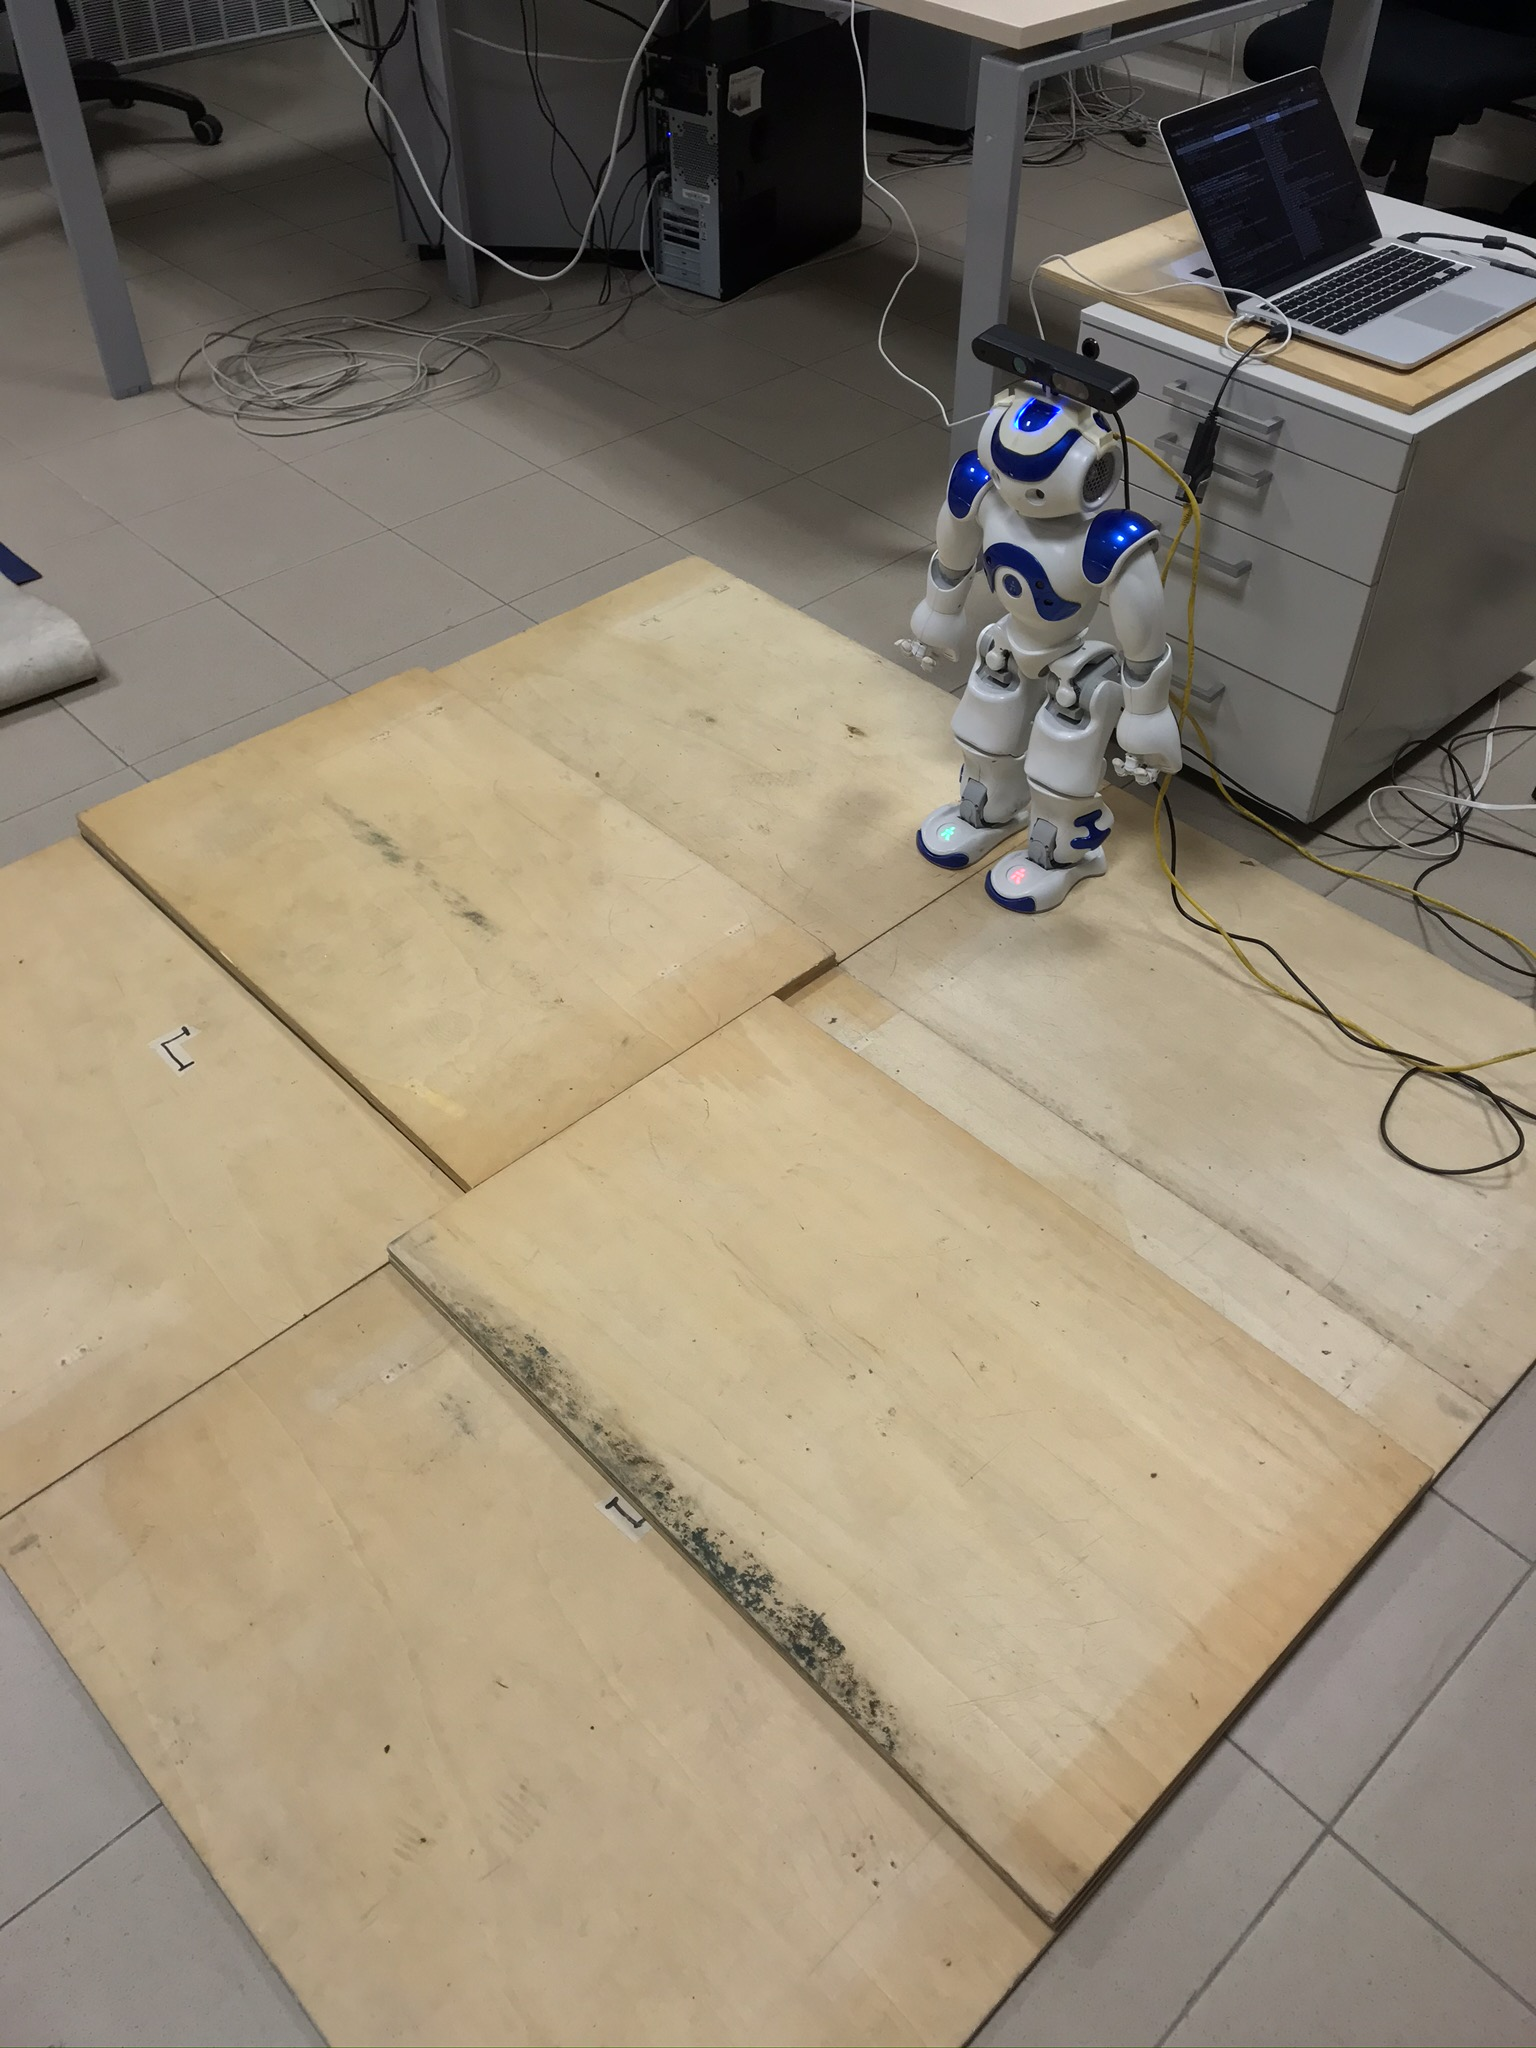
\includegraphics[width=\textwidth]{figures/NAO-with-xtion-full-env.JPEG}
    \caption{}
    \label{fig:nao-with-xtion-full-env}
  \end{subfigure}
  \caption{On the left, NAO humanoid robot with ASUS Xtion Pro placed on top.
      On the right, NAO humanoid robot in the environment described in
			Section \ref{sec:stair-climbing-unkenv}, 
      right before starting the execution of the experiment.}
\end{figure}
\begin{figure}
  \centering
  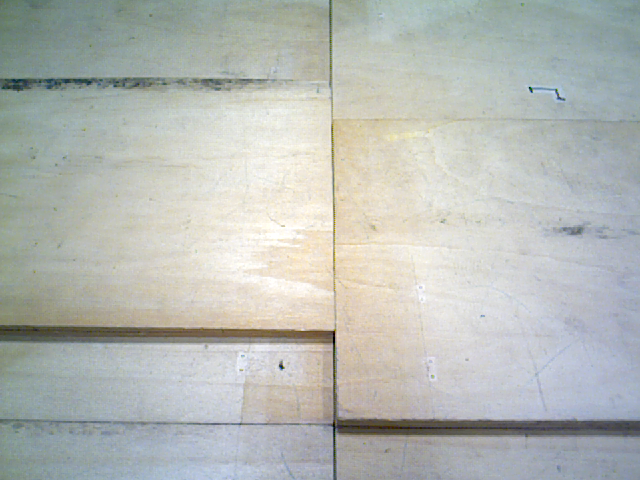
\includegraphics[width=0.85\textwidth]{figures/xtion_rgb_20cm.png}
  \caption{RGB image seen by the ASUS Xtion Pro placed on top of the robot.
      The corresponding depth image is sent to \texttt{elevation\_mapping}
      to build the map.}
  \label{fig:xtion-rgb-20cm}
\end{figure}
\begin{figure}
  \centering
  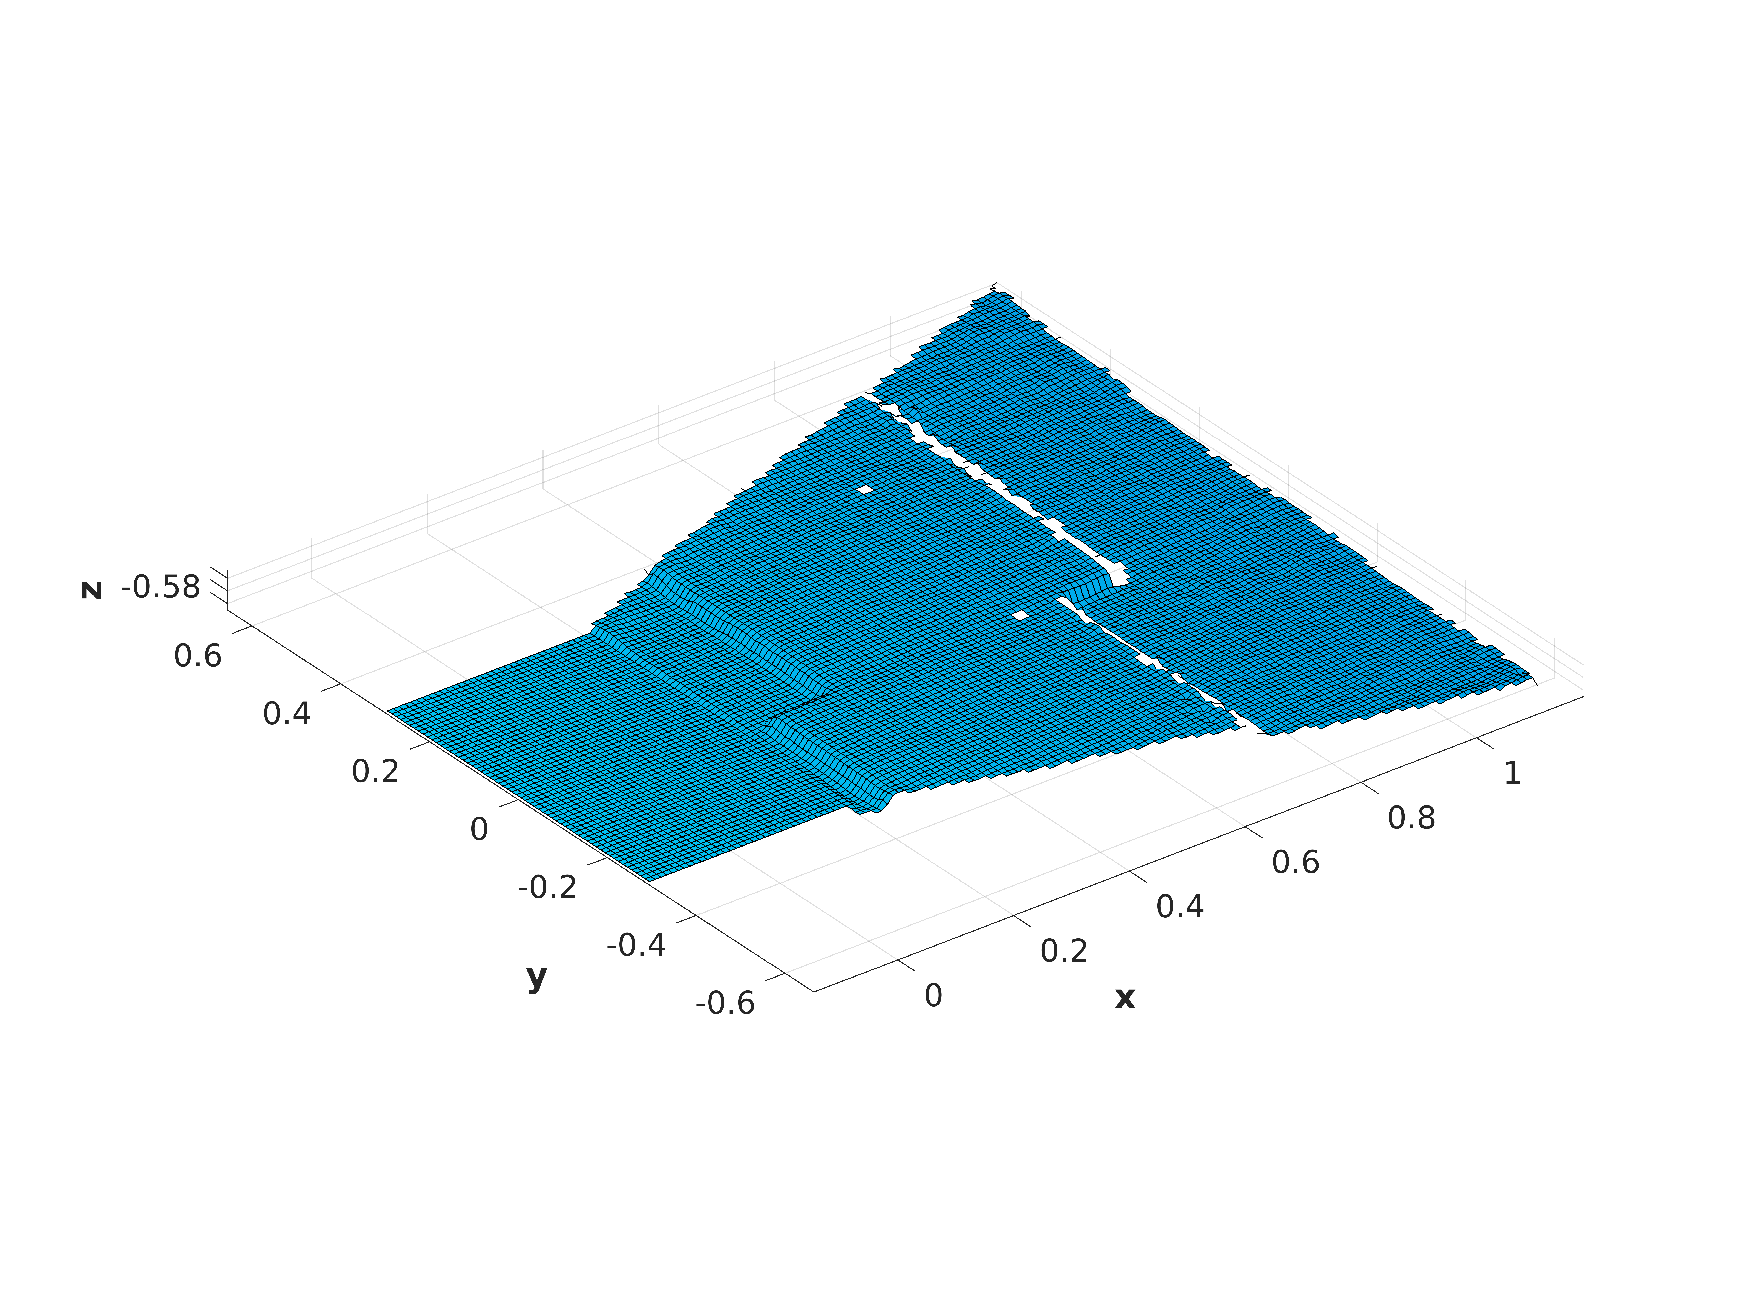
\includegraphics[width=\textwidth]{figures/onlymap-xtion-20cm.pdf}
  \caption{Elevation map build by \texttt{elevation\_mapping} for the scenario 
      ``Stair Climbing in Unknown Environment'' described in section 
      \ref{sec:stair-climbing-unkenv}.}
  \label{fig:onlymap-xtion-20cm}
\end{figure}

